%\title{LaTeX Portrait Poster Template}
%%%%%%%%%%%%%%%%%%%%%%%%%%%%%%%%%%%%%%%%%
% a0poster Portrait Poster
% LaTeX Template
% Version 1.0 (22/06/13)
%
% The a0poster class was created by:
% Gerlinde Kettl and Matthias Weiser (tex@kettl.de)
% 
% Adapter by Jens Buysse for Hogeschool Gent
% This template has been downloaded from:
% http://www.LaTeXTemplates.com
%
% License:
% CC BY-NC-SA 3.0 (http://creativecommons.org/licenses/by-nc-sa/3.0/)
%
%%%%%%%%%%%%%%%%%%%%%%%%%%%%%%%%%%%%%%%%%

%----------------------------------------------------------------------------------------
%	PACKAGES AND OTHER DOCUMENT CONFIGURATIONS
%----------------------------------------------------------------------------------------

\documentclass[a0,portrait]{a0poster}

\usepackage{multicol} % This is so we can have multiple columns of text side-by-side
\columnsep=100pt % This is the amount of white space between the columns in the poster
\columnseprule=3pt % This is the thickness of the black line between the columns in the poster

\usepackage[svgnames]{xcolor} % Specify colors by their 'svgnames', for a full list of all colors available see here: http://www.latextemplates.com/svgnames-colors

\usepackage{times} % Use the times font
%\usepackage{palatino} % Uncomment to use the Palatino font

\usepackage{graphicx} % Required for including images
\graphicspath{{figures/}} % Location of the graphics files
\usepackage{booktabs} % Top and bottom rules for table
\usepackage[font=small,labelfont=bf]{caption} % Required for specifying captions to tables and figures
\usepackage{amsfonts, amsmath, amsthm, amssymb} % For math fonts, symbols and environments
\usepackage{wrapfig} % Allows wrapping text around tables and figures
\usepackage[export]{adjustbox}

\begin{document}

%----------------------------------------------------------------------------------------
%	POSTER HEADER 
%----------------------------------------------------------------------------------------

% The header is divided into two boxes:
% The first is 75% wide and houses the title, subtitle, names, university/organization and contact information
% The second is 25% wide and houses a logo for your university/organization or a photo of you
% The widths of these boxes can be easily edited to accommodate your content as you see fit

\begin{minipage}[t]{0.75\linewidth}
\VeryHuge \color{HoGentAccent1} \textbf{Een vergelijkende studie van NLP-platformen voor het bouwen van een chatbot met een sterk begrijpend vermogen en lage foutenmarge} \color{Black}\\ % Title
\Huge\textit{}\\[2.4cm] % Subtitle
\huge \textbf{Deschacht Jarne, Helsens Kenny, Lewyllie Liesbeth}\\[0.5cm] % Author(s)
\huge Hogeschool Gent, Valentin Vaerwyckweg 1, 9000 Gent\\[0.4cm] % University/organization
\Large \texttt{jarne.deschacht@student.hogent.be} \\
\end{minipage}
%
\begin{minipage}[t]{0.25\linewidth}

\includegraphics[width=13cm,right]{figures/HOGENT_Logo_Pos_rgb.png} 

\end{minipage}

\vspace{1cm} % A bit of extra whitespace between the header and poster content

%----------------------------------------------------------------------------------------

\begin{multicols}{2} % This is how many columns your poster will be broken into, a portrait poster is generally split into 2 columns

%----------------------------------------------------------------------------------------
%	ABSTRACT
%----------------------------------------------------------------------------------------

\color{HoGentAccent1} % Navy color for the abstract

\begin{abstract}
\noindent Chatbots zijn tegenwoordig niet meer weg te denken uit onze maatschappij. We beseffen
het niet altijd, maar we hebben meer interactie met een chatbot dan dat we initieel zouden
verwachten. Denk hierbij bijvoorbeeld aan de klantenservice van bedrijven, want het
gebeurt niet vaak meer dat ons eerste contact direct met een menselijke medewerker is als
we bijvoorbeeld een chatbericht sturen naar de klantenservice van een bedrijf. Meestal is
er een geautomatiseerde gesprekspartner geïmplementeerd om de klant verder te helpen
bij problemen en vragen. Bedrijven gaan tegenwoordig vaak hun eigen chatbots bouwen,
maar hoe moet dat juist? De ontwikkelingen binnen de wereld van artificiële intelligentie
zijn de laatste jaren enorm sterk toegenomen. Deze ontwikkelingen bieden bedrijven
de mogelijkheid om daarop in te spelen en er zelf mee te werken. Het implementeren
van een chatbot vanaf het begin is een erg complex proces dat veel tijd en kennis vereist.
Verschillende bedrijven hebben hierop ingespeeld door platformen te ontwikkelen die de
implementatie van een chatbot vergemakkelijken. Hierdoor kunnen bedrijven, waar er
onvoldoende kennis en tijd is voor de implementatie van chatbots, toch een chatbot bouwen
en gebruiken. Er zijn tal van bedrijven die hun eigen chatbotplatformen hebben ontwikkeld
waarmee eenvoudig een chatbot opgezet kan worden. Bedrijven zoals Google, Facebook,
Microsoft, IBM, Amazon, etc. hebben allemaal zo’n platform gebouwd, maar welk van
deze platformen is de beste?
\end{abstract}
%----------------------------------------------------------------------------------------
%	INTRODUCTION
%----------------------------------------------------------------------------------------

\begin{center}\vspace{1cm}
    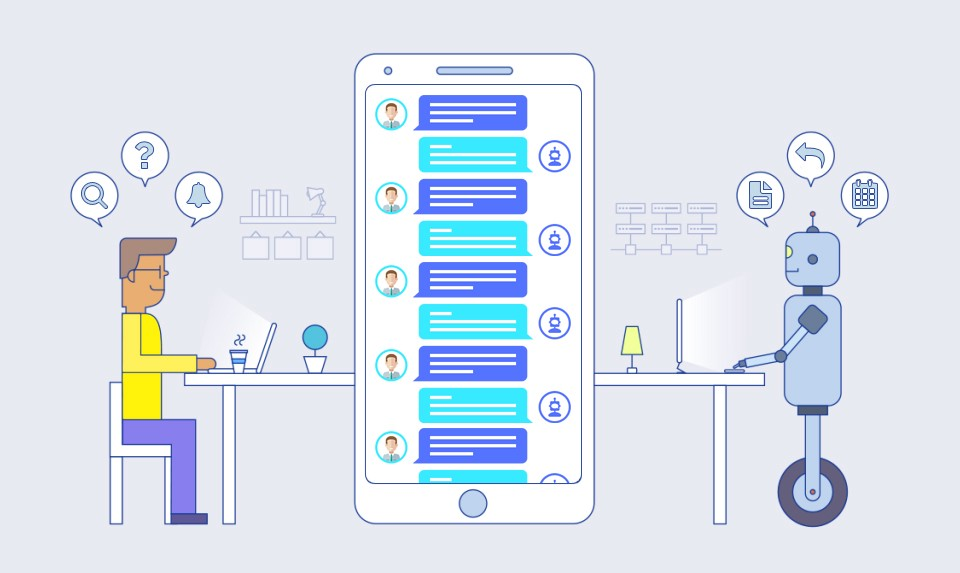
\includegraphics[width=1.0\linewidth]{human-machine}
    \captionof{figure}{\color{HoGentAccent5} Visualisatie van een digitale conversatie tussen mens en chatbot. Bron:  https://chatbotslife.com/chatbots-the-importance-of-chatbots-in-every-business-bf178bc9cfef}
\end{center}\vspace{1cm}

\bigskip
\bigskip

\color{HoGentAccent1} 
\section*{Introductie}
\color{black}
\color{black}

Binnen deze bachelorproef is er een uitgebreid onderzoek gevoerd naar de verschillende
gratis platformen die overweg kunnen met de Nederlandse taal, de meest interessante
werden verder uitgediept. Daarbij werd er stilgestaan bij de verschillende functionaliteiten,
de voor- en nadelen, de werking, de prestaties en de verschillende integratiemogelijkheden,
zoals bijvoorbeeld met Slack of Facebook Messenger. De focus binnen deze bachelorproef
lag op het vinden van het platform die het best verstaat wat de gebruiker juist bedoeld en
ook belangrijke informatie zoals datums, locaties, tijdstippen, etc. kan extraheren. Daarbij
werd ook rekening gehouden met spellingsfouten. De platformen zijn door middel van
objectieve beoordelingstechnieken en verschillende experimenten getest.

%----------------------------------------------------------------------------------------
%	GEOLOGY
%----------------------------------------------------------------------------------------

\color{Black} % DarkSlateGray color for the rest of the content
\color{HoGentAccent1} 
\section*{Experimenten}
\color{black}
Om een vergelijking te kunnen maken van het begrijpend vermogen van de platformen,
vonden er drie experimenten plaats waarbij er op een objectieve manier beoordeeld
werd. Er werd een dataset opgesteld waarmee alle platformen getraind en
geëvalueerd werden. Op deze manier kregen alle platformen exact dezelfde informatie
en kon er objectief beoordeeld worden. Er werd telkens een deel van de dataset gebruikt
om de chatbots te trainen en het andere deel diende voor het testen. Er werden drie verschillende experimenten uitgevoerd die onafhankelijk van elkaar de verschillende platformen beoordeelden. Daarbij werd duidelijk welk platform het best verstaat wat de gebruiker juist bedoeld, welk platform het best parameterwaarden zoals datums, locaties, tijdstippen, etc. kan extraheren en welk platform het beste om kan met taalfouten.

%------------------------------------------------



\color{HoGentAccent1} 
\section*{Conclusies}
\color{black}
Het resultaat is dat het platform van Facebook (Wit.ai) algemeen de beste resultaten kan
voorleggen. Zowel bij het correct verstaan van berichten als bij het afleiden van belangrijke
informatie, scoort deze het sterkst. Het nadeel van Wit.ai is dat het moeite heeft met
spellingsfouten en scoort daarbij minder goed in vergelijking met zijn concurrenten. IBM
Watson kan hier de beste resultaten voorleggen. Ook de ingebouwde integratiemogelijkheden
van andere platformen zijn geavanceerder dan die van Wit.ai, daarbij is Dialogflow de
koploper met een grote verscheidenheid aan integraties.
%----------------------------------------------------------------------------------------
%	FORTHCOMING RESEARCH
%----------------------------------------------------------------------------------------
\color{HoGentAccent1} 
\section*{Toekomstig onderzoek}
\color{black}
Deze bachelorproef biedt veel mogelijkheden tot verder onderzoek, doordat de beoordeling
werd beperkt tot de Nederlandse taal en doordat er geen betaalde platformen onderzocht
werden. De dataset die werd gebruikt, is ook fictief en te klein om perfect representatief te
zijn. Een onderzoek met een grotere representatieve dataset zou hier een oplossing voor
kunnen bieden. Dit onderzoek is alvast een goed startpunt.


%----------------------------------------------------------------------------------------

\end{multicols}
\end{document}